\documentclass[12pt,a4paper,numbers=enddot,headings=small]{scrartcl} %article
\usepackage[utf8]{inputenc}
\usepackage[T1]{fontenc}
\usepackage{microtype}
\usepackage[polish]{babel}
\usepackage[parfill]{parskip}
\usepackage{xcolor}

\usepackage{amsmath}
\usepackage{amssymb}
\usepackage{graphicx}
\usepackage{float}

\usepackage{tabularx}
\usepackage{makecell}
\usepackage[linkbordercolor={1 1 1}, colorlinks, urlcolor=teal, linkcolor=teal]{hyperref}

\usepackage{caption}
\captionsetup[figure]{name=Rys., labelsep=period}
\usepackage[none]{hyphenat}

\begin{document}
	
	.
	\vspace{3cm}
	\large Biologically Inspired Artificial Inteligence
	\begin{center}
		{
			\vspace{5cm}
			\huge \bfseries
			Klasyfikacja i rekonstrukcja \\
			obrazów z sygnału EEG
			\bigskip
			
			\large
			Raport z projektu
		}
	\end{center}
	
	\vfill		%\vspace{11cm}
	
	{\large
		\emph{Paulina Kędzierska}\\
		\emph{Szymon Konarski}
		
		\rightline{22.08.2026}
		
	}
	
	\newpage
	
	\section{Cel projektu}
	
	Celem projektu było sprawdzenie, czy modele sztucznej inteligencji są w stanie sklasyfikować i odtworzyć obrazy wyłącznie na podstawie danych EEG. W tym celu zapoznano się z procedurą badania z zakresu neurobiologii oraz przeanalizowano dostępne dane. Następnie odpowiednio przygotowano je do wykorzystania przez wybrany model sieci neuronowej i przeprowadzono próby klasyfikacji oraz rekonstrukcji obrazów. Cały przebieg projektu, poczynione obserwacje oraz wyciągnięte wnioski zostały przedstawione w niniejszym raporcie.
	
	\section{Założenia}
	
	\subsection{Struktura danych}
	
	W badaniu wykorzystano obrazy należące do 11 kategorii: abstrakt, samolot, jabłko, banan, ptak, łódź, samochód, pies, osoba, pociąg oraz zebra. Kategoria abstrakt różniła się od pozostałych, ponieważ zamiast zdjęć zawierała prostą grafikę złożoną z figur geometrycznych.
	
	W każdej kategorii znajdowało się 20 obrazów, co dawało łącznie 220 unikalnych obrazów. Zestaw ten był prezentowany w sześciu seriach, więc każdy obraz pojawiał się podczas badania sześć razy. W efekcie dla jednego badanego otrzymano łącznie 1320 prób, czyli po 220 prób w każdej serii.
	
	Każda próba miała przypisany numer serii oraz numer próby. W pliku z zapisanymi zdarzeniami znajdowały się również informacje o czasie wystąpienia danego zdarzenia oraz jego rodzaju. Dzięki temu można było później określić, kiedy dokładnie pojawił się konkretny obraz i jaki fragment sygnału EEG odpowiadał jego prezentacji.
	
	Takie uporządkowanie danych było szczególnie istotne z punktu widzenia dalszej analizy. Pozwalało ono połączyć sygnał EEG z konkretnym obrazem i jego kategorią, a także rozdzielić poszczególne etapy pojedynczej próby.
	
	\subsection{Przebieg badania}
	
	Przed rozpoczęciem właściwego badania uczestnik uzupełniał krótką ankietę oraz otrzymał instrukcję dotyczącą przebiegu eksperymentu. Następnie wykonano krótki etap przygotowawczy, w którym rejestrowano aktywność EEG przy zamkniętych oczach, a później przy otwartych oczach. Po tym etapie rozpoczęła się właściwa część badania.
	
	Badanym był student realizujący projekt, który przed rozpoczęciem eksperymentu nie miał dostępu do obrazów wykorzystywanych podczas badania. Uczestnik miał założony czepek EEG z elektrodami, a jego zadaniem było skupienie wzroku na wyświetlanych obrazach i późniejsze ich opisanie.
	
	Każda próba przebiegała według tego samego schematu:
	
	\begin{center}
		\textit{fiksacja $\rightarrow$ czarny ekran $\rightarrow$ obraz $\rightarrow$ czarny ekran $\rightarrow$ opis obrazu $\rightarrow$ naciśnięcie spacji $\rightarrow$ czarny ekran}
	\end{center}
	
	Na początku pojawiał się punkt fiksacji, na którym badany miał skupić wzrok. Następnie na krótko wyświetlany był czarny ekran, po którym pojawiał się właściwy obraz. Obraz był prezentowany przez około 0,5 sekundy.
	
	Po obejrzeniu każdego obrazu uczestnik miał w jednym zdaniu opisać to, co zobaczył. Kiedy kończył opis, naciskał klawisz spacji. W tym momencie zapisywane było zdarzenie \texttt{SPACE\_PRESSED}, a następnie pojawiał się krótki czarny ekran i rozpoczynała się kolejna próba.
	
	Poszczególne etapy były zapisywane w pliku z wykorzystaniem specjalnych znaczników. Przykładowo, \texttt{FIXATION} oznaczało rozpoczęcie fiksacji, \texttt{IMAGE\_ON} moment pojawienia się obrazu, \texttt{DESCRIBE\_SCREEN} rozpoczęcie etapu opisu, a \texttt{SPACE\_PRESSED} zakończenie opisu przez badanego. Dzięki temu późniejsza analiza nie wymagała zgadywania, w którym momencie prezentowany był dany obraz.
	
	Całe badanie zostało podzielone na sześć serii po 220 prób. Pomiędzy seriami uczestnik miał przerwy, dzięki czemu mógł odpocząć przed rozpoczęciem kolejnej części badania. Łączny czas rejestracji wyniósł około 2,5 godziny, wliczając przygotowanie, przerwy oraz poszczególne etapy badania.
	
	Czas potrzebny na wykonanie pojedynczej próby nie był zawsze taki sam. Sama prezentacja obrazu trwała około 0,5 sekundy, natomiast etap opisywania zależał od badanego i od tego, ile czasu potrzebował on na przygotowanie odpowiedzi. Z tego powodu poszczególne serie trwały różną ilość czasu.
	
	Po zakończeniu głównej części eksperymentu przeprowadzono również etap końcowy, obejmujący ankietę po badaniu. Pozwoliło to zebrać dodatkowe informacje dotyczące udziału w eksperymencie, niezwiązane bezpośrednio z samym zapisem EEG.
	
	W rezultacie otrzymano zbiór danych zawierający zarówno sygnał EEG, jak i informacje o dokładnym przebiegu eksperymentu. Dzięki zapisanym znacznikom zdarzeń możliwe jest określenie, kiedy uczestnik oglądał konkretny obraz, kiedy go opisywał oraz kiedy zakończył daną próbę. Stanowi to podstawę do dalszego przetwarzania i analizy zebranych danych.
	
	\section{Użyte środowisko programistyczne, biblioteki i narzędzia}
	
	\subsection{Środowisko programistyczne}
	
	\textcolor{red}{PyCharm, Terminal linuxowy (po zainstalowaniu pyhona3, potrzebnych pakietów i bibliotek na systemie operacyjnym Ubuntu), Google Colab (powiedźmy, że to środowisko programistyczne :p).}
	
	\subsection{Biblioteki}
	
	\textcolor{red}{m.in. MNE, matplotlib, pandas, numpy, sklearn.}
	
	\subsection{Narzędzia}
	
	\textcolor{red}{Tu może być tak naprawdę cokolwiek: gen AI, które nam pomagało (Gemini, Claude, ChatGPT), jakieś napisane przez nas skrypty albo inne fajne rzeczy, które nie są jedną z tych trzech innych kategori w tym podrozdziale.}
	
	\subsection{Sieci neuronowe}
	
	\textcolor{red}{Użyte przez nas finalnie sieci neuronowe. Można tu też wspomnieć o tych, które rozważaliśmy, ale ostatecznie z jakiegoś powodu odrzuciliśmy.}
	
	\section{Przygotowanie danych}
	
	Miejsce na opis naszego pipelinu przygotowującego dane do wrzucenia ich potem modelowi. Skupiłabym się tu na tym finalnym i ewentualnie dopisała, jak ten pipeline zmieniał się na przestrzeni semestru.
	
	\subsection{Wczytanie surowych danych}
	
	\subsection{Mapowanie kanałów}
	
	Kolejnym krokiem przygotowania danych było uporządkowanie informacji o kanałach. W tym celu jednolicono ich nazwy, przypisano im odpowiednie typy oraz określono położenie elektrod zgodnie z międzynarodowym standardem 10--20.
	
	Standard 10--20 (ang. \emph{international 10--20 system}) to jeden ze sposobów rozmieszczania i nazywania elektrod na powierzchni głowy. Jego nazwa wynika ze sposobu wyznaczania pozycji elektrod: rozmieszcza się je w odstępach stanowiących około 10\% lub 20\% odległości pomiędzy charakterystycznymi punktami anatomicznymi głowy -- nasion (zagłębienie u nasady nosa), inion (guzowatość potyliczna) oraz punktami przedusznymi po obu stronach głowy. Dzięki temu możliwe jest stosowanie podobnego układu elektrod niezależnie od kształtu i rozmiaru głowy badanego, co ułatwia porównywanie wyników uzyskanych dla różnych osób.
	
	Nazwa każdej elektrody koduje jej położenie. Litera (lub zestaw liter) wskazuje jej położenie na powierzchni głowy: 
	
	\begin{itemize}
		\item \texttt{Fp} -- okolice czołowo-biegunową,
		\item \texttt{F} -- czołową,
		\item \texttt{C} -- centralną,
		\item \texttt{T} -- skroniową,
		\item \texttt{P} -- ciemieniową,
		\item \texttt{O} -- potyliczną.
	\end{itemize}
	
	W standardzie mogą występować również oznaczenia pośrednie, takie jak \texttt{FC}, \texttt{CP} czy \texttt{PO}, jednak nie odnotowano ich dla opisywanego badania. 
	
	Liczby nieparzyste oznaczają lewą stronę głowy, a parzyste prawą. Im większa liczba, tym dalej od linii środkowej znajduje się elektroda. Litera \texttt{z} (od ang. \emph{zero}) oznacza położenie na linii środkowej. Przykładowo, \texttt{Fp1} oznacza elektrodę znajdującą się po lewej stronie w okolicy czołowo-biegunowej, \texttt{Fp2} -- jej odpowiednik po prawej stronie, natomiast elektroda \texttt{Cz} leży centralnie na linii środkowej. W niniejszym badaniu szczególnie istotne były elektrody \texttt{O1} i \texttt{O2}, znajdujące się odpowiednio po lewej i prawej stronie w okolicy potylicznej, ponieważ rejestrowana aktywność była związana m.in. z odpowiedzią kory wzrokowej.
	
	Przygotowanie kanałów przebiegało w kilku krokach, których kod przedstawiono na rys.~\ref{fig:channel_mapping}.
	
	\begin{figure}[H]
		\centering
		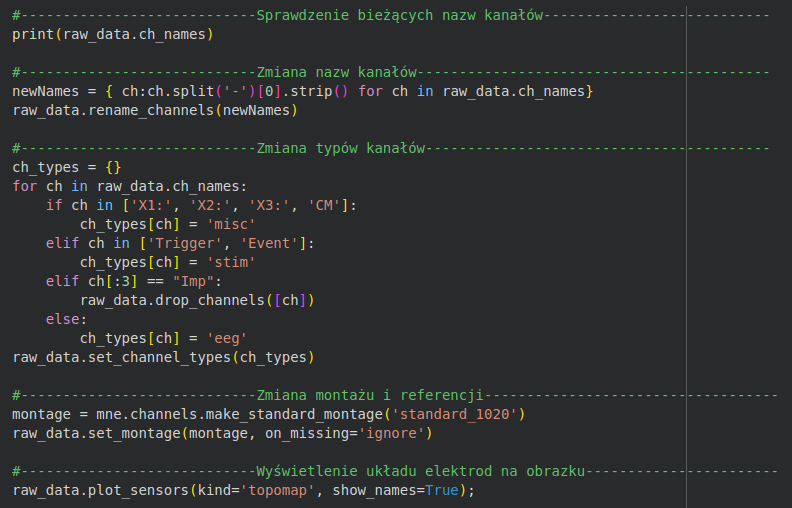
\includegraphics[width=1.0\textwidth]{assets/channel_mapping.png}
		\caption{Fragment kodu pipeline'u przygotowującego dane, odpowiedzialny za mapowanie kanałów na standard \texttt{standard\_1020}.}
		\label{fig:channel_mapping}
	\end{figure}
	
	Na początku wyświetlono bieżące nazwy kanałów, aby sprawdzić ich postać przed rozpoczęciem dalszego przetwarzania. Następnie ujednolicono nazwy poprzez usunięcie fragmentów znajdujących się po znaku \texttt{-}. W tym celu wykorzystano funkcję \texttt{split()}, która pozwoliła pozostawić pierwszą część każdej nazwy. Przykładowo, \texttt{Fp1-REF} zostało zmienione na \texttt{Fp1}. W przypadku kanałów zawierających dwukropek, np. \texttt{X1:} lub \texttt{Ax:}, znak ten pozostawał częścią nazwy.
	
	Następnie każdemu kanałowi przypisano odpowiedni typ. Elektrody EEG oznaczono jako \texttt{eeg}, kanały pomocnicze -- wejścia analogowe \texttt{X1}-\texttt{X3} oraz elektrodę trybu wspólnego \texttt{CM} -- jako \texttt{misc}, a kanały ze znacznikami zdarzeń (\texttt{Trigger}, \texttt{Event}) jako \texttt{stim}. Kanały zawierające pomiary impedancji (o nazwach rozpoczynających się od \texttt{Imp}) usunięto, ponieważ nie niosą informacji przydatnej w dalszej analizie.
	
	Podział kanałów na poszczególne typy był istotny podczas dalszego przetwarzania danych, ponieważ kolejne operacje, takie jak montaż, filtrowanie czy analiza ICA, domyślnie obejmują wyłącznie kanały typu \texttt{eeg}. Kanały \texttt{misc} przechowują dodatkowe informacje, które nie są traktowane jak sygnał mózgowy, natomiast kanały \texttt{stim} pozwalały określić moment wystąpienia poszczególnych zdarzeń. Z tego powodu kanały \texttt{misc} i \texttt{stim} nie zostały wycięte ze zbioru danych, tylko jedynie odpowienio oznaczone.
	
	Po uporządkowaniu kanałów przypisano do danych montaż \texttt{standard\_1020}. Wykorzystano w tym celu funkcję \texttt{make\_standard\_montage()}, a następnie \texttt{set\_montage()}. Montaż zawiera informacje o przestrzennym położeniu elektrod, dzięki czemu nazwy kanałów, mogły zostać powiązane z ich pozycjami na głowie. Parametr \texttt{on\_missing='ignore'} pozwolił na pominięcie kanałów, dla których nie znaleziono odpowiedniej pozycji w standardzie 10-20, bez zgłaszania błędu.
	
	Poprawność przypisania montażu sprawdzono za pomocą funkcji \texttt{plot\_sensors(
	\\kind='topomap', show\_names=True)}. Wynik przedstawiono na rys.~\ref{fig:standard_10-20_map}.
	
	\begin{figure}[H]
		\centering
		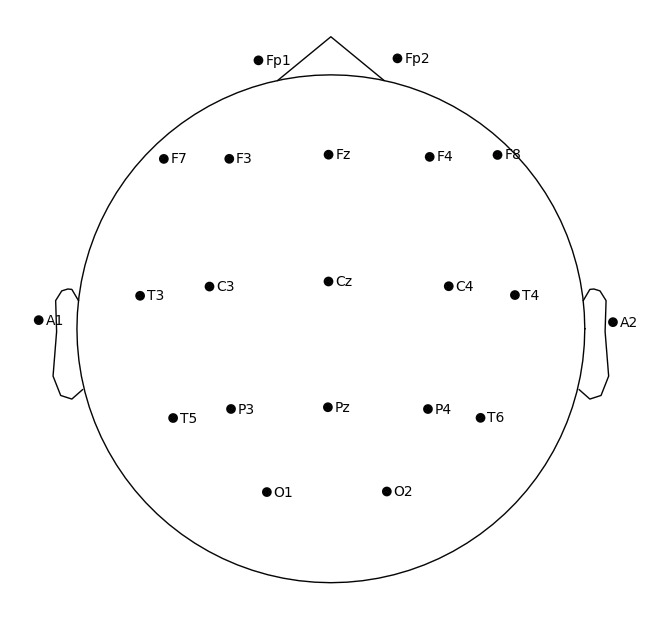
\includegraphics[width=0.9\textwidth]{assets/standard_10-20_map.png}
		\caption{Rozmieszczenie elektrod EEG po przypisaniu montażu \texttt{standard\_1020}.}
		\label{fig:standard_10-20_map}
	\end{figure}
	
	Na wykresie elektrody EEG zostały rozmieszczone zgodnie ze standardem 10--20. Widoczna jest symetria układu względem linii środkowej głowy oraz podział elektrod na lewą i prawą stronę. Kanały pomocnicze nie są przedstawione jako elektrody na mapie, ponieważ nie mają przypisanych pozycji w zastosowanym montażu. Uzyskany wynik potwierdził poprawność przypisania nazw elektrod do standardowych pozycji przestrzennych. Przygotowane w ten sposób dane mogły zostać wykorzystane w kolejnych etapach analizy.
	
	\subsection{Ciąg dalszy :pp}
	
	\section{Klasyfikacja obrazów}
	
	\textcolor{red}{Jak ją zrobiliśmy i co wyszło.}
	
	\section{Rekonstrukcja obrazów}
	
	\textcolor{red}{Jak ją zrobiliśmy i co wyszło.}
	
	\section{Podsumowanie projektu - uwagi i wnioski}
	
	\textcolor{red}{Jaka wyszła nam zgodność, co może być tego przyczyną i ewentualnie inne cenne uwagi.}
	
\end{document}